\section[Wineland the Good]{
    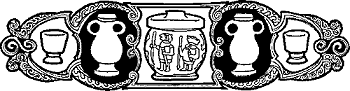
\includegraphics[width=9.3cm]{viking-tales/044}\\
    Wineland the Good}

\lettrine{O}{n} an autumn, a year or two after Leif came home, Eric and
his men saw two large ships come to land not far down the shore from the
house.

``They look like trading ships,'' Eric said. ``Let us go down to see
them.''

``I will go, too,'' Gudrid said. ``Perhaps they will have rich cloth and
jewelry. It is long since I had my eyes on a new dress.''

So they all went down and found two large trading ships lying in the
water. A great many men were on the shore making a fire.

``Welcome to Greenland!'' called Eric. ``What are your names and your
country?''

Then a fine, big man walked out from among the men and went up to Eric.

``I am Thorfinn,'' he said, ``a trader. I sailed this summer from
Iceland with forty men and a shipload of goods. On the sea I met this
other ship from Iceland. The master is Biarni. Come and look at my
goods.''

So he rowed Eric and Gudrid out and they went aboard his boat. Thorfinn
opened his chests and showed Eric gleaming swords and bracelets and axes
and farm tools. But before Gudrid he spread beautiful cloth and gold
embroidery and golden necklaces. As they looked, he told of doings in
Iceland and asked of Greenland.

``We never see such things as these in this bare land,'' Gudrid said, as
she smoothed a beautiful dress of purple velvet. ``I envy the women of
Iceland their fair clothes.''

``There is no need of that,'' Thorfinn said, ``for this dress is yours
and anything else from my chests that you like. Here is a necklace that
I beg you to take. It did not have a fairer mistress in Greece where I
got it.''

``You are a very generous trader,'' Gudrid said.

Then Thorfinn gave Eric a great sword with a gold-studded scabbard.
After a while he took them to Biarni's ship. He also gave them gifts.
They all talked and laughed much while they were together.

``You are merry comrades,'' Eric said. ``I ask you both and all your men
to spend the winter at my house. You can put your goods into my
storehouses.''

``By my sword! a generous offer,'' said Thorfinn. ``As for me, I am
happy to come.''

Biarni and all the rest said the same thing. Thorfinn walked to the
house with Eric and Gudrid, while the other men sailed to the ship-sheds
and pulled their boats under them.

Then Thorfinn saw to the unloading and storing of his goods.

``Is this Gudrid your daughter?'' he asked of Eric one day.

``She is the widow of my son Thorstein,'' Eric said. ``He died the same
winter that they were married. Her father, too, died not long ago. So
Gudrid lives with me.''

Now all that winter until Yule-time Eric spread a good feast every
night. There was laughter through his house all the time. Often at the
feasts the men cast lots to see whether they might sit on the
cross-bench with the women. Sometimes it was Thorfinn's luck to sit by
Gudrid. Then they talked gaily and drank together.

At last Yule was coming near. Eric went about the house gloomy then. One
day Thorfinn put his hand on Eric's shoulder and said:

``Something is troubling you, Eric. We have all noticed that you are not
gay as you used to be. Tell me what is the matter.''

``You have carried yourselves like noble men in my house,'' Eric
answered. ``I am proud to have you for guests. Now I am ashamed that you
should not find a house worthy of you. I am ashamed that when you leave
me you will have to say that you never spent a worse Yule than you did
with Eric the Red in Greenland. For my cupboards are empty.''

``Oh, that is easily mended,'' Thorfinn said. ``No house could feed
eighty men so long and not feel it. I never knew so generous a host
before. But I have flour and grain and mead in my boat. You are welcome
to all of it. You have only to open the doors of your own storehouses.
It is a little gift.''

So Eric used those things, and there was never a merrier Yule feast than
in his house that winter.

When Yule was over, Thorfinn said to Eric:

``Gudrid is a beautiful and wise woman. I wish to have her for my
wife.''

``You seem to be a man worthy of her,'' Eric said.

So that winter Gudrid and Thorfinn were married and lived at Eric's
house.

One day Thorfinn said to Eric:

``I have heard much of this wonderful Wineland since I have been here.
It seems to me that it is worth while to go and see more of it.''

``My son Thorstein and I tried it once,'' said Eric. ``It was the year
after Leif came back. We set out with a fair ship and with glad hearts,
but we tossed about all summer on the sea and got nowhere. We were wet
with storm, lean with hunger and illness, and heartsick at our bad
luck.''

``And yet,'' Thorfinn said, ``another time we might have better weather.
I have never seen so fair a land as this seems to be.''

Then he went to Leif and talked long with him. Leif told him in what
direction he had sailed to come home, and how the shores looked that he
had passed.

``I think I could find my way,'' Thorfinn said. ``My heart moves me to
try this frolic.''

He spoke to Gudrid about it.

``Oh, yes!'' she cried. ``Let us go. It is long since I felt a boat
leaping under me. I am tired of sitting still. I want to feel the warm
days and see the soft grass and the high trees and taste the grapes of
this Wineland the Good.''

Then he talked with his men and with Biarni.

``We are ready,'' they all said. ``We are only waiting for a leader.''

``Then let us go!'' cried Thorfinn.

So in the spring they fitted up their two ships and put into them
provisions and a few cattle. Some of Eric's men also got ready a boat,
so that three ships set sail from Eric's harbor carrying one hundred and
sixty men to Wineland. As they started, Gudrid stood on the deck and
sang:

\begin{quote}
``I will feast my eyes on new things--\\
On mighty trees and purple grapes,\\
On beds of flowers and soft grass.\\
I will sun myself in a warm land.''
\end{quote}

They sailed on and past those shores that Leif had spoken of. Whenever
they saw any interesting place they sailed in and looked about and
rested there.

They had gone far south, past many fair shores with woods on them, when
Gudrid said one day:

``This is a beautiful bay with a smooth, green field by it, and the
great mountains far back. I should like to stay there for a little
while.''

So they sailed in and drew their ships up on shore. They put up the
awnings in them.

``These shall be our houses,'' Thorfinn said.

They were strange-looking houses--shining dragons with gay backs lying
on the yellow sand. Near them the Norsemen lighted fires and cooked
their supper. That night they slept in the ships. In the morning Gudrid
said:

``I long to see what is back of that mountain.''

So they all climbed it. When they stood on the top they could see far
over the country.

``There is a lake that we must see,'' Thorfinn said.

``I should like to sail around that bay,'' said Biarni, pointing.

``I am going to walk up that valley yonder,'' one of the men said.

And everyone saw some place where he would like to go. So for all that
summer they camped in that spot and went about the country seeing new
things. They hunted in the woods and caught rabbits and birds and
sometimes bears and deer. Every day some men rowed out to sea and
fished. There was an island in the bay where thousands of birds had
their nests. The men gathered eggs here.

``We have more to eat than we had in Greenland or Iceland,'' Thorfinn
said, ``and need not work at all. It is all play.''

Near the end of summer Thorfinn spoke to his comrades.

``Have we not seen everything here? Let us go to a new place. We have
not yet found grapes.''

Thorfinn and Biarni and all their men sailed south again. But some of
Eric's men went off in their boat another way. Years afterward the
Greenlanders heard that they were shipwrecked and made slaves in
Ireland.

After Thorfinn and Biarni had sailed for many days they landed on a low,
green place. There were hills around it. A little lake was there.

``What is growing on those hillsides?'' Thorfinn said, shading his eyes
with his hand.

He and some others ran up there. The people on shore heard them shout.
Soon they came running back with their hands full of something.

``Grapes! Grapes!'' they were shouting.

All those people sat down and ate the grapes and then went to the
hillside and picked more.

``Now we are indeed in Wineland,'' they said. ``It is as wonderful as
Leif's stories. Surely we must stay here for a long time.''

The very next day they went into the woods and began to cut out lumber.
The huts that they built were little things. They had no windows, and in
the doorways the men hung their cloaks instead of doors.

``We can be out in the air so much in this warm country,'' said Gudrid,
``that we do not need fine houses.''

The huts were scattered all about, some on the side of the lake, some at
the shore of the harbor, some on the hillside. Gudrid had said:

``I want to live by the lake where I can look into the green woods and
hear sweet bird-noises.''

So Thorfinn built his hut there.

As they sat about the campfire one night, Biarni said:

``It is strange that so good a land should be empty. I suppose that
these are the first houses that were ever built in Wineland. It is
wonderful to think that we are alone here in this great land.''

All that winter no snow fell. The cattle pastured on the grass.

``To think of the cold, frozen winters in Greenland!'' Gudrid said.
``Oh! this is the sun's own land.''

In the beginning of that winter a little son was born to Gudrid and
Thorfinn.

``A health to the first Winelander!'' the men shouted and drank down
their wine; for they had made some from Wineland grapes.

``Will he be the father of a great country, as Ingolf was?'' Biarni
mused.

Gudrid looked at her baby and smiled.

``You will be as sunny as this good land, I hope,'' she said.

They named him Snorri. He grew fast and soon crept along the yellow
sand, and toddled among the grapevines, and climbed into the boats and
learned to talk. The men called him the ``Wineland king.''

``I never knew a baby before,'' one of the men said.

``No,'' said another. ``Swords are jealous. But when they are in their
scabbards, we can do other things, even play with babies.''

``I wonder whether I have forgotten how to swing my sword in this quiet
land,'' another man said.

One spring morning when the men got up and went out from their huts to
the fires to cook they saw a great many canoes in the harbor. Men were
in them paddling toward shore.

``What is this?'' cried the Norsemen to one another. ``Where did they
come from? Are they foes? Who ever saw such boats before? The men's
faces are brown.''

``Let every man have his sword ready,'' cried Thorfinn. ``But do not
draw until I command. Let us go to meet them.''

So they went and stood on the shore. Soon the men from the canoes landed
and stood looking at the Norsemen. The strangers' skin was brown. Their
faces were broad. Their hair was black. Their bodies were short. They
wore leather clothes. One man among them seemed to be chief. He spread
out his open hands to the Norsemen.

``He is showing us that he has no weapons,'' Biarni said. ``He comes in
peace.''

Then Thorfinn showed his empty hands and asked:

``What do you want?''

The stranger said something, but the Norsemen could not understand. It
was some new language. Then the chief pointed to one of the huts and
walked toward it. He and his men walked all around it and felt of the
timber and went into it and looked at all the things there--spades and
cloaks and drinking-horns. As they looked they talked together. They
went to all the other huts and looked at everything there. One of them
found a red cloak. He spread it out and showed it to the others. They
all stood about it and looked at it and felt of it and talked fast.

``They seem to like my cloak,'' Biarni said.

One of the strangers went down to their canoes and soon came back with
an armload of furs--fox-skins, otter-skins, beaver-skins. The chief took
some and held them out to Thorfinn and hugged the cloak to him.

\begin{figure}
    \centering
    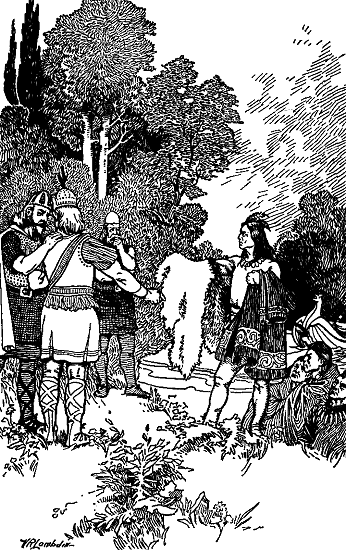
\includegraphics[width=9.1cm]{viking-tales/045}
    \caption{``The chief held them out to Thorfinn and hugged the cloak
        to him''}
\end{figure}

``He wants to trade,'' Thorfinn said. ``Will you do it, Biarni?''

``Yes,'' Biarni answered, and took the furs.

``If they want red stuff, I have a whole roll of red cloth that I will
trade,'' one of the other men said.

He went and got it. When the strangers saw it they quickly held out more
furs and seemed eager to trade. So Thorfinn cut the cloth into pieces
and sold every scrap. When the strangers got it they tied it about their
heads and seemed much pleased.

While this trading was going on and everybody was good-natured, a bull
of Thorfinn's ran out of the woods bellowing and came towards the crowd.
When the strangers heard it and saw it they threw down whatever was in
their hands and ran to their canoes and paddled off as fast as they
could.

The Norsemen laughed.

``We have lost our customers,'' Biarni said.

``Did they never see a bull before?'' laughed one of the men.

Now after three weeks the Norsemen saw canoes in the bay again. This
time it was black with them, there were so many. The people in them were
all making a horrible shout.

``It is a war-cry,'' Thorfinn said, and he raised a red shield. ``They
are surely twenty to our one, but we must fight. Stand in close line and
give them a taste of your swords.''

Even as he spoke a great shower of stones fell upon them. Some of the
Norsemen were hit on the head and knocked down. Biarni got a broken arm.
Still the storm came fast. The strangers had landed and were running
toward the Norsemen. They threw their stones with sling-shots, and they
yelled all the time.

``Oh, this is no kind of fighting for brave men!'' Thorfinn cried
angrily.

The Norsemen's swords swung fast, and many of the strangers died under
them, but still others came on, throwing stones and swinging stone axes.
The horrible yelling and the strange things that the savages did
frightened the Norsemen.

``These are not men,'' some one cried.

Then those Norsemen who had never been afraid of anything turned and
ran. But when they came to the top of a rough hill Thorfinn cried:

``What are we doing? Shall we die here in this empty land with no one to
bury us? We are leaving our women.''

Then one of the women ran out of the hut where they were hiding.

``Give me a sword!'' she cried. ``I can drive them back. Are Norsemen
not better than these savages?''

Then those warriors stopped, ashamed, and stood up before the wild men
and fought so fiercely that the strangers turned and fled down to their
canoes and paddled away.

``Oh, I am glad they are gone!'' Thorfinn said. ``It was an ugly
fight.''

``Thor would not have loved that battle,'' one said.

``It was no battle,'' another replied. ``It was like fighting against an
army of poisonous flies.''

The Norsemen were all worn and bleeding and sore. They went to their
huts and dressed their wounds, and the women helped them. At supper that
night they talked about the fight for a long time.

``I will not stay here,'' Gudrid said. ``Perhaps these wild men have
gone away to get more people and will come back and kill us. Oh! they
are ugly.''

``Perhaps brown faces are looking at us now from behind the trees in the
woods back there,'' said Biarni.

It was the wish of all to go home. So after a few days they sailed back
to Greenland with good weather all the way. The people at Eric's house
were very glad to see them.

``We were afraid you had died,'' they said.

``And I thought once that we should never leave Wineland alive,''
Thorfinn answered.

Then they told all the story.

``I wonder why I had no such bad luck,'' Leif said. ``But you have a
better shipload than I got.''

He was looking at the bundles of furs and the kegs of wine.

``Yes,'' said Thorfinn, ``we have come back richer than when we left.
But I will never go again for all the skins in the woods.''

The next summer Thorfinn took Gudrid and Snorri and all his people and
sailed back to Iceland, his home. There he lived until he died. People
looked at him in wonder.

``That is the man who went to Wineland and fought with wild men,'' they
said. ``Snorri is his son. He is the first and last Winelander, for no
one will ever go there again. It will be an empty and forgotten land.''

And so it was for a long time. Some wise men wrote down the story of
those voyages and of that land, and people read the tale and liked it,
but no one remembered where the place was. It all seemed like a fairy
tale. Long afterwards, however, men began to read those stories with
wide-open eyes and to wonder. They guessed and talked together, and
studied this and that land, and read the story over and over. At last
they have learned that Wineland was in America, on the eastern shore of
the United States, and they have called Snorri the first American, and
have put up statues of Leif Ericsson, the first comer to
America.\footnote{See note about eskimos on page~\pageref{eskimos}.}

\begin{figure}[hb]
    \centering
    \vskip8pt
    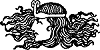
\includegraphics[width=2.7cm]{viking-tales/017}
\end{figure}
